\documentclass[../../main.tex]{subfiles}

\begin{document}

\section{Introduction to Algorithm Engineering}
\subsection{Analyzing slide 15}
Here is slide 15 again:

~\\
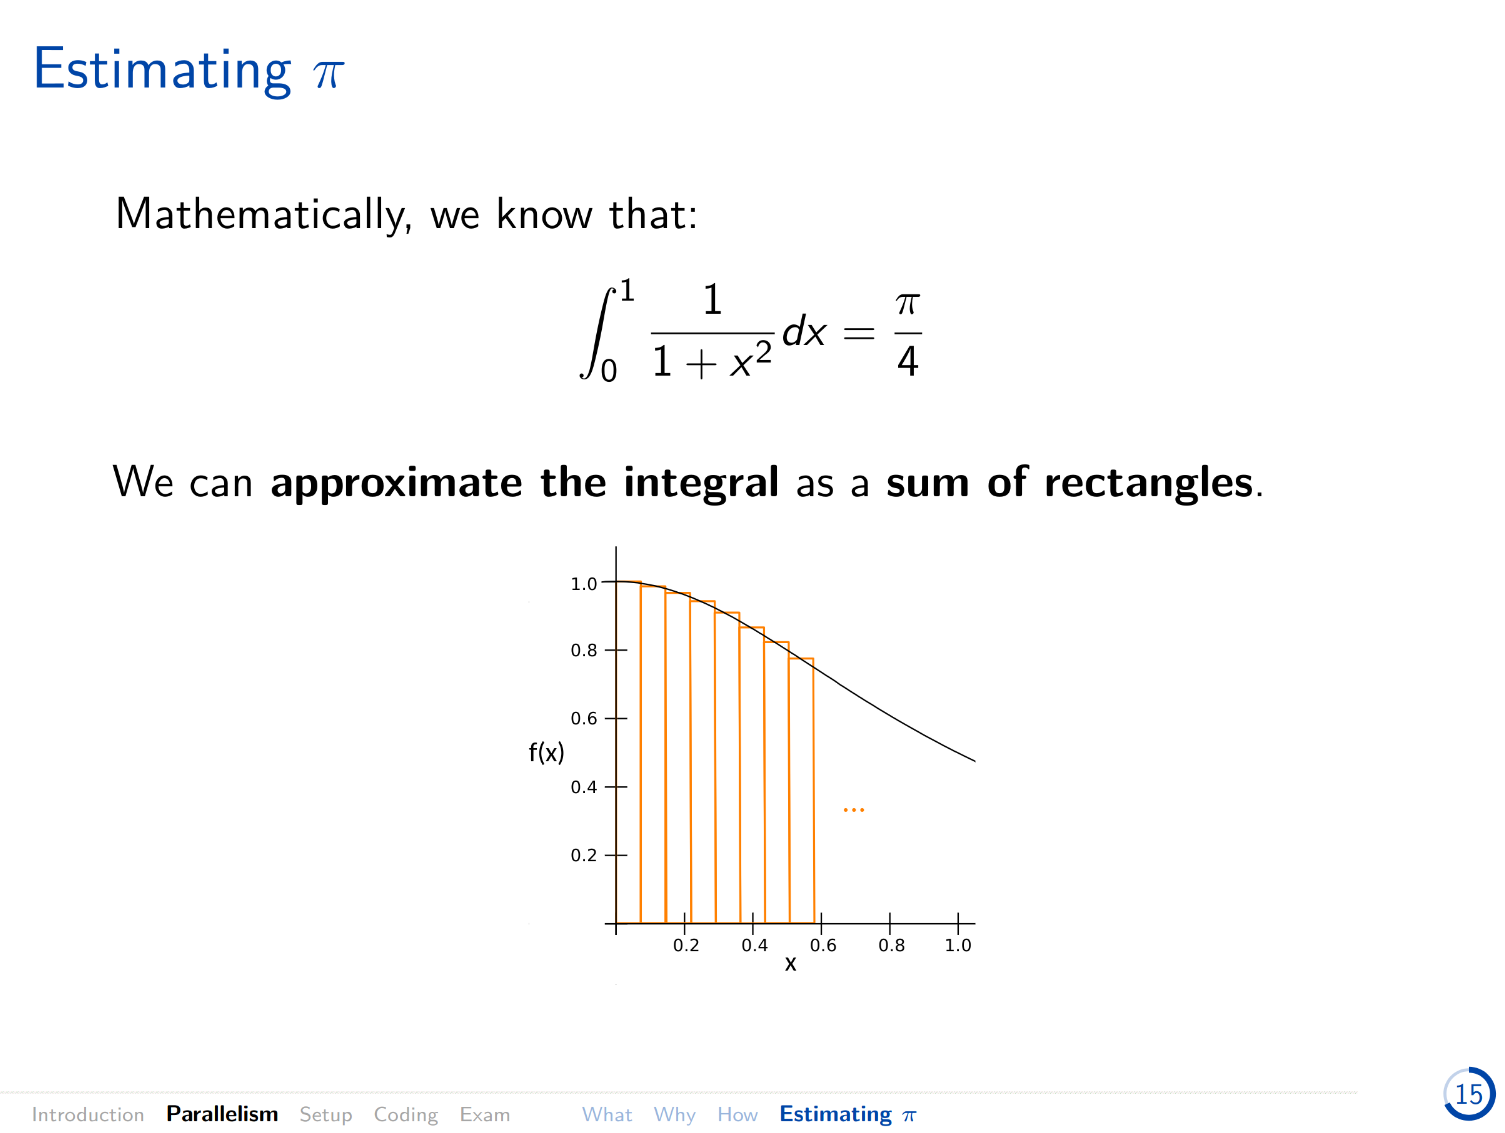
\includegraphics[width=\textwidth]{page_15.png}

~\\
Let us proof the satement
\[
    \int_{0}^{1}\frac{1}{1+x^2} dx = \frac{\pi}{4}
\]

\noindent using
\[
    (f^{-1})'(x_0) = \frac{1}{f'(f^-1(x_0))} \ \ \ \ \ :
\]

\begin{proof}
    Let \( \tan : (- \frac{\pi}{2}, \frac{\pi}{2}) \rightarrow \mathbb R \) be the usual trigonometric function.
    Clearly, it is a bijection, and hence its inverse function \( \arctan : \mathbb R \rightarrow (- \frac{\pi}{2}, \frac{\pi}{2}) \) exists.
    Now, let us argue with the above identity:
    \[
        \arctan'(x_0) = \frac{1}{\tan'(\arctan(x_0))} = \cos^2(\arctan(x_0)) \ \ \ \ \ ,
    \]

    \noindent
    where we have used that \(\tan'(x_0) = \frac{1}{\cos^2(x_0)}\).
    (This can easily be derived by the chain and product rule, knowing the derivatives of \(\sin , \cos \) and \(\frac{1}{x}\), as well as the fact that \(\tan(x)=\frac{\sin(x)}{\cos(x)}\).)
    
    \noindent
    Now, we would like to transform \(\cos^2(\bullet)\) into something like foo\((\tan(\bullet))\), such that $\tan$ and $\arctan$ would cancel.
    Luckily, we can do this using the trigonometric identity

    \begin{align*}
    &\sin^2 + \cos^2 = 1 \\
    \Leftrightarrow \ &\tan^2 \cos^2 + \cos^2 = 1 \\
    \Leftrightarrow \ &(\tan^2 + 1) \cos^2 = 1 \\
    \Leftrightarrow \ &\cos^2 = \frac{1}{\tan^2 + 1}
    \end{align*}


    ~\\
    \noindent
    Plugging this into our equation yields

    \[
        \arctan'(x_0) = \frac{1}{\tan^2(\arctan(x_0)) + 1} \ \ \ \ \ .
    \]

    ~\\
    But by the definition of $\arctan$, we get

    \[
        \arctan'(x_0) = \frac{1}{x_0^2 + 1} \ \ \ \ \ .    
    \]

    ~\\
    Thus, we have established that $\arctan$ is an antiderivative of $\frac{1}{x^2 + 1}$.
    \\
    By the fundamental theorem of calculus we get

    \[
        \int_{0}^{1}\frac{1}{1+x^2} dx = \arctan(1) - \arctan(0) \ \ \ \ \ .
    \]

    ~\\
    Now note that \(0, \frac{\pi}{4} \in (- \frac{\pi}{2}, \frac{\pi}{2})\), and \(\tan(0) = 0\), \(\tan(\frac{\pi}{4}) = 1\).
    In other words, we have \(\arctan(0) = 0\),  \(\arctan(1) = \frac{\pi}{4}\). Thus,

    \[
        \int_{0}^{1}\frac{1}{1+x^2} dx = \frac{\pi}{4} \ \ \ \ \ .
    \]

\end{proof}

~\\
The reason we established this equation in the first place is because it allows for a simple approximation for $\pi$.
We do this by using numerical methods for approximating integrals.

One way to do this is to calculate the Riemann sum, as shown in the lecture.
The Riemann sum tries to approximate little intervals of the function $\frac{1}{1+x^2}$ by constant functions.
A better way to approximate the function on these intervals would be a linear function connecting the end points, resulting in the \em Trapezoidal Rule\em.

Even better is the approximation by parabolas, which pass through the end points of the interval as well as the mid point. This is called the \em Simpson Rule\em.
It reads as follows:
\[
    \int_{t}^{t+h} f(x) dx \ \approx \ \frac{h}{6} \Big[ f(t) + 4f(t+\frac{h}{2}) + f(t+h) \Big] \ \ \ \ \ .
\]

~\\
When approximating an integral by splitting it into smaller intervals, we use the following formula.
To this end, let $P$ be such a partition. Then

\[
    \int_{a}^{b} f(x) dx \ \ \approx \sum_{(t, t+h) \in P} I_{(t, t+h)}(f) \ \ \ \ \ ,
\]

where \(I_{(t, t+h)}(f)\) tries to approximate \(\int_{t}^{t+h} f(x) dx\).

~\\
Combining these results, one might get even faster convergence.
But note that machines might have trouble dealing with very small numbers, thus this process should be used with caution.

~\\
\subsection{Chapter 1 from Computer Systems: A Programmer's Perspective}
The book gave a quick overview about operating systems and computer hardware, and the flow of execution.
I'd like to discuss the memory hierarchy as well as virtual memory.

\subsubsection{Memory Hierarchy}
The inverse correlation between speed and volume of different memory types war presented in the book.
This lead to the memory hierarchy, where we try exploit the benefits of both worlds be having big, slow memory, and a smaller amount of fast memory, which we the computer tries to employ as much as possible.

~\\
Two reasons for this are
\begin{enumerate}
    \item Increased physical memory cells: More logical memory requires more physical memory cells. These cells need to be connected to control circuits, and larger memory arrays result in longer signal paths and higher capacitance. This increases signal propagation delay, making the memory slower.
    \item Heat production: Larger memory volumes consume more power, and the switching of many transistors generates more heat. Excessive heat can degrade performance and force memory to operate at lower speeds to prevent overheating.
\end{enumerate}

~\\
\subsubsection{Virtual Memory}
One of the core principles in mathematics and computer science is abstraction.
The operating system provides such an abstraction in form of I/O communication, running multiple programs concurrently using processes, and translating virtual addresses into physical ones.

This is very interesting, as by doing so, two distinct processes are unable to access the other ones data.
To illustrate this, imagine you write a simple C program, create a pointer, print the pointer location, write an integer there based on a command line argument, and print the content periodically.
If one now starts two instances of the program, one where it writes a 1, another one with 0, they won't interfere with one another, the first process will always read a 1, the second one 0.

Behind the scenes, the operating system works together with the \em memory management unit\em, which translates every address the program uses to its real address before accessing.
And exactly this translation process is program specific.
Hence, the operating system successfully abstracted the memory.

~\\
\newpage
\subsection{Parallelizing "Estimating $\pi$ using Monte Carlo"}
Here is the parallelized version of the code:

\smallbreak
\smallbreak
\begin{samepage}
\begin{lstlisting}
#include <iostream>
#include <omp.h>
#include <random>

using namespace std;

int main() {
    
    int n = 100000000; // number of points to generate
    int counter = 0; // counter for points lying in the first quadrant of a unit circle
    auto start_time = omp_get_wtime(); // omp_get_wtime() is an OpenMP library routine

    // compute n points and test if they lie within the first quadrant of a unit circle
    #pragma omp parallel
    {
        default_random_engine re{(size_t) omp_get_thread_num()};
        uniform_real_distribution<double> zero_to_one{0.0, 1.0};

        int local_counter = 0;
        int local_n = (n / omp_get_num_threads()) + ((n % omp_get_num_threads() > omp_get_thread_num()) ? 1 : 0);
        for (int i = 0; i < local_n; ++i) {
            auto x = zero_to_one(re); // generate random number between 0.0 and 1.0
            auto y = zero_to_one(re); // generate random number between 0.0 and 1.0
            if (x * x + y * y <= 1.0) { // if the point lies in the first quadrant of a unit circle
                ++local_counter;
            }
        }
        #pragma omp atomic
        counter += local_counter;
    }

    auto run_time = omp_get_wtime() - start_time;
    auto pi = 4 * (double(counter) / n);

    cout << "pi: " << pi << endl;
    cout << "run_time: " << run_time << " s" << endl;
    cout << "n: " << n << endl;
}
\end{lstlisting}
\end{samepage}
\end{document}
